\documentclass[11pt, oneside]{article} 
\usepackage{styleBase}				% packages and definitions for base style
\usepackage{styleCode}				% packages and definitions for code style

\title{SAS handbook}
\author{Colton Gearhart}
\date{January 30, 2019}							

\begin{document}
\maketitle
\tableofcontents
\newpage

\section{Read in data}

\subsection{Input data}

Datalines:
\begin{itemize}
\item Used to read data that you enter directly in the program.
\item The DATALINES statement is used with an INPUT statement.
\item Can add an INFILE statement if need additional SAS instructions to read the desired data.
\item Must be the last statement in the DATA step and immediately precedes the first data line.
\item Use a null statement (a single semicolon) to indicate the end of the input data. 
\end{itemize}
\lstinputlisting{ReadData-Datalines.txt}
\begin{figure}[H]
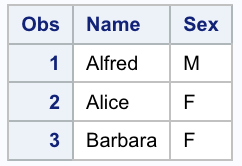
\includegraphics[scale=0.6]{ReadData-Datalines.png}
\end{figure}

Infile:
\begin{itemize}
\item Used to read data from an external source.
\item Files can be txt, csv, etc. (may need extra options depending on source type).
\item Can also use a FILENAME statement (outside of the DATA step) to specify data file.
\end{itemize}
\lstinputlisting{ReadData-Infile.txt}
\begin{figure}[H]
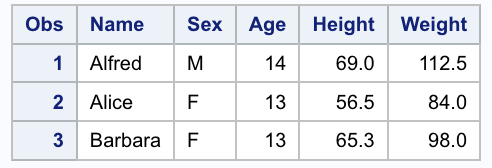
\includegraphics[scale=0.6]{ReadData-Infile.png}
\\\footnotesize{* Output for proc import as well.}
\end{figure}

Proc import:
\begin{itemize}
\item Another way to read to read data from an external source.
\item Can be used for most file types, but it could result in data errors.
\item Note -> xlsx files cannot be read in using an INFILE statement, so have to us PROC IMPORT.
\end{itemize}
\lstinputlisting{ReadData-ProcImport.txt}

Types of input styles:
\begin{itemize}
\item Modified list input
	\begin{itemize}
	\item Allows you to read list input with nonstandard data by using SAS informats.
	\item Uses a scanning method for locating data values.
	\item Data values must be separated by at least one blank (or other defined delimiter).
	\item Do not have to specify the location of the data fields.
	\end{itemize}
\item Formatted input
	\begin{itemize}
	\item Enables you to read nonstandard data values that are aligned in columns in the data records.
	\item Typically used with pointer controls that enable you to control the position of the input pointer in the input buffer when you read data.
	\end{itemize}
\end{itemize}

\subsection{Options}

Here are some common options used with INFILE statement...

DLM=\textit{'list-of-delimiting-characters'}:
\begin{itemize}
\item Specifies an alternate delimiter.
\end{itemize}

DSD (delimiter-sensitive data):
\begin{itemize}
\item Use when you want to treat two consecutive delimiters as a missing value.
\item Also specifies that when data values are enclosed in quotation marks, delimiters within the value are treated as character data.
\item Use the tilde (\textasciitilde) format modifier to retain the quotation marks.
\end{itemize}

Firstobs=\textit{record number}:
\begin{itemize}
\item Specifies the first record for SAS to begin reading the input data records.
\end{itemize}

Obs=\textit{record number}:
\begin{itemize}
\item Specifies the last record for SAS to end reading the input data records.
\end{itemize}

Missover:
\begin{itemize}
\item Use if the last field or fields might be missing and you want SAS to assign missing values to the corresponding variable.
\end{itemize}

N=\textit{available-lines}:
\begin{itemize}
\item Specifies the number of lines that are available to the input pointer at one time.
\item When using \# pointer controls in an INPUT statement, include a \# pointer control that equals the value of the N= option (even if no data is read from that record).
\end{itemize}
    
\subsection{Modifiers}

\& (ampersand):
\begin{itemize}
\item Enables you to read character values that contain embedded blanks.
\item SAS reads until it encounters two consecutive blanks or the defined length of the variable, whichever comes first.
\end{itemize}
\lstinputlisting{ReadData-Ampersand.txt}
\begin{figure}[H]
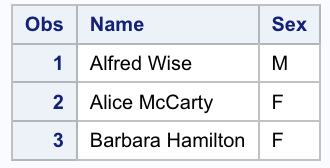
\includegraphics[scale=0.6]{ReadData-Ampersand.png}
\end{figure}

: (colon):
\begin{itemize}
\item Enables you to specify an informat, whether character or numeric.
\item SAS reads the defined length of the variable or until it encounters a blank column, whichever comes first.
\end{itemize}
\lstinputlisting{ReadData-Colon.txt}
\begin{figure}[H]
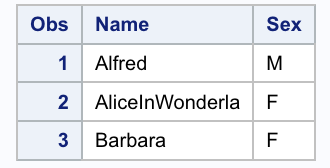
\includegraphics[scale=0.6]{ReadData-Colon.png}
\end{figure}

@ (trailing @):
\begin{itemize}
\item Holds an input record for the execution of the next INPUT statement \textbf{within the same iteration} of the DATA step.
\item Use when you want to read multiple records from the same line of data.
\item Can add an indicator (counter) variable for each record.
\item The trailing @ must be the last item in the INPUT statement.
\end{itemize}
\lstinputlisting{ReadData-TrailingAt.txt}
\begin{figure}[H]
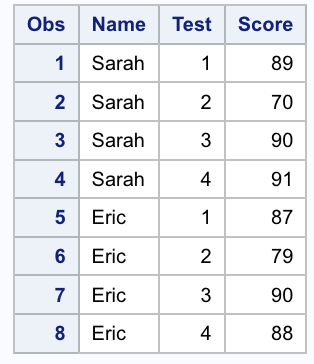
\includegraphics[scale=0.6]{ReadData-TrailingAt.png}
\end{figure}

@@ (double trailing @):
\begin{itemize}
\item Holds the input record for the execution of the next INPUT statement \textbf{across iterations} of the DATA step (i.e. there is an implicit output once all the input variables have been read, so @@ holds the record between multiple outputs).
\item Use when have more than one record per line within raw data file.
\item The double trailing @ must be the last item in the INPUT statement.
\end{itemize}
\lstinputlisting{ReadData-DoubleTrailingAt.txt}
\begin{figure}[H]
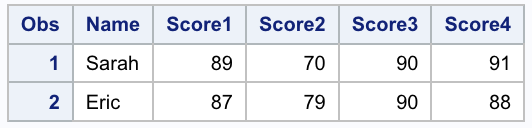
\includegraphics[scale=0.6]{ReadData-DoubleTrailingAt.png}
\end{figure}

@n and +n (column pointer controls):
\begin{itemize}
\item @n moves the pointer to column $n$ (use when columns have nonstandard lengths).
\item +n moves the pointer $n$ columns (use when columns have standard lengths).
\item Note -> $n$ can also be a numeric variable, expression, character string, etc.
\end{itemize}
\lstinputlisting{ReadData-ColumnPointerControls.txt}
\lstinputlisting{ReadData-LinePointerControls.txt}
\begin{figure}[H]
	\begin{minipage}{0.3\textwidth}
		\centering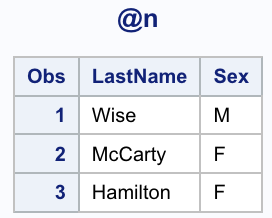
\includegraphics[scale=0.6]{ReadData-LinePointerControls-AtN}
	\end{minipage}
	\begin{minipage}{0.3\textwidth}
		\centering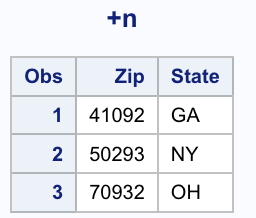
\includegraphics[scale=0.6]{ReadData-LinePointerControls-PlusN}
	\end{minipage}
\end{figure}

\#n (line pointer controls):
\begin{itemize}
\item \#n moves the pointer to record $n$ (i.e. jumps to $n$th line in the raw data for the current record).
\item Use when data for a single record is on multiple lines.
\item Note -> $n$ can also be a numeric variable or expression.
\end{itemize}
\lstinputlisting{ReadData-LinePointerControls.txt}
\begin{figure}[H]
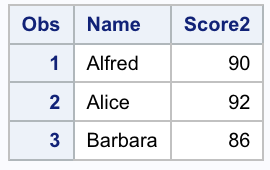
\includegraphics[scale=0.6]{ReadData-LinePointerControls.png}
\end{figure}

? and ?? (error reporting modifiers):
\begin{itemize}
\item ? suppresses printing the invalid data note when SAS encounters invalid data values.
\item ?? suppresses printing the messages and the input lines when SAS encounters invalid data values.
\end{itemize}

\subsection{Informats}

\begin{itemize}
\item Describe the data value and tells SAS how to convert it.
\item Can be specified in the INPUT statement or in an INFORMAT statement (using the INFORMAT statement tells SAS to use the informat in any subsequent input statements).
\end{itemize}
\lstinputlisting{ReadData-Informats.txt}
\begin{figure}[H]
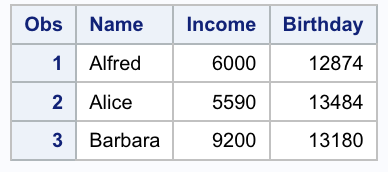
\includegraphics[scale=0.6]{ReadData-Informats.png}
\end{figure}

\section{Data step stuff}

\subsection{Drop, keep and rename variables}

Dropping, keeping and renaming variables:
\begin{itemize}
\item Can do these by using a statement, dataset option or both.
\item Results depend on if you specify the data set options on an input or an output data set.
\item Order of application in SAS -> For input datasets, drop= and keep= options, then rename= option, then drop and keep statements, then rename statement, then options again for output datasets.
\item Statements:
	\begin{itemize}
	\item Apply to output data sets only.
	\item Affect all output data sets.
	\item Can be used in DATA steps only.
	\item Can appear anywhere in DATA steps (although rename must be after keep / drop).
	\end{itemize}
\item Dataset options:
	\begin{itemize}
	\item Apply to output or input data sets.
	\item Affect individual data sets.
	\item Can be used in DATA steps and PROC steps.
	\item Must immediately follow the name of each data set to which they apply.
	\end{itemize}
\item Shorthand notation -> Can use numbered range lists (i.e. x1,x2,...,xn = x1-xn).
\end{itemize}
\lstinputlisting{DataStep-DropKeepRen-General.txt}
\lstinputlisting{DataStep-DropKeepRen-Example.txt}
\begin{figure}[H]
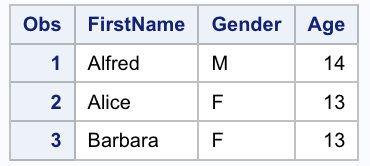
\includegraphics[scale=0.6]{DataStep-DropKeepRen.png}
\end{figure}
	
\subsection{Formats and labels}

Formats:
\begin{itemize}
	\item Change the appearance of a variable?s value in a report.
	\item The values stored in the data set are not changed.
	\item Remove a format by specifying a format statement (with desired variables) after the input dataset.
\end{itemize}

Labels:
\begin{itemize}
	\item Change the appearance of a variable's name in a report.
	\item Have to add a label option in PROC PRINT to apply them.
\end{itemize}

\lstinputlisting{DataStep-FormatsLabels.txt}
\begin{figure}[H]
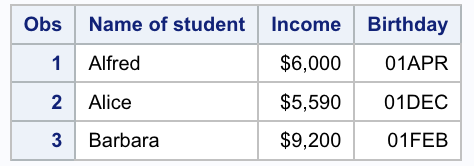
\includegraphics[scale=0.6]{DataStep-FormatsLabels.png}
\end{figure}
\lstinputlisting{DataStep-FormatsLabels-Removed.txt}
\begin{figure}[H]
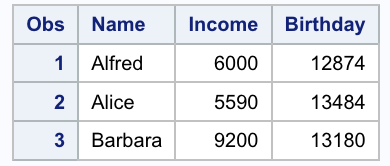
\includegraphics[scale=0.6]{DataStep-FormatsLabels-Removed.png}
\end{figure}

\subsection{Conditional logic statements}

\lstinputlisting{DataStep-Conditional-General.txt}
\lstinputlisting{DataStep-Conditional-Example.txt}
\begin{figure}[H]
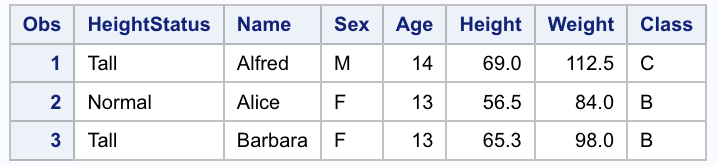
\includegraphics[scale=0.6]{DataStep-Conditional.png}
\end{figure}

\subsection{Do loops}

\lstinputlisting{DataStep-DoLoops.txt}

\subsection{Retain statement}

\begin{itemize}
\item Retains the value of the variable across iterations of the data step.
\item Initializes the retained variable to missing or a specified initial value before the first iteration of the data step.
\item Use when you want to create an accumulating variable (or a counter variable).
	\begin{itemize}
	\item If accumulating a variable and one observation has a missing value, the rest of the observations for the accumulating variable will be missing.
	\item So have to use SUM function.
	\end{itemize}
\item Using the shorthand notation \textit{accumvar}+\textit{varinterest}, the accumulating variable is initialized to zero and automatically retained.
\end{itemize}
\lstinputlisting{DataStep-Retain-General.txt}
\lstinputlisting{DataStep-Retain-Example.txt}
\begin{figure}[H]
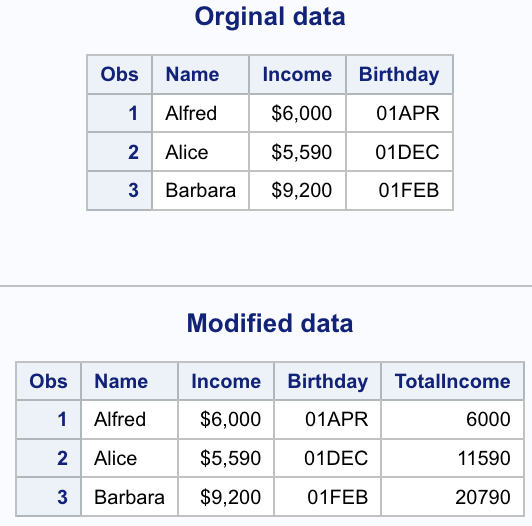
\includegraphics[scale=0.6]{DataStep-Retain.png}
\end{figure}

\subsection{Arrays}
	
\begin{itemize}
\item Temporary grouping of SAS variables that are arranged in a particular order.
\item Identified by an array name.
\item Must contain all numeric or all character variables.
\item Exists only for the duration of the current DATA step (is not a variable).
\item If variables associated with an array do not exist, SAS creates them.
\end{itemize}

Tips:
\begin{itemize}
\item Helpful when systematically recoding data in many variables (e.g. missing data).
\item When the initial value list is specified, all elements behave as if they were named in a RETAIN statement (i.e. this creates a lookup table).
\item You can use the keyword \_TEMPORARY\_ in an ARRAY statement to indicate that the elements are not needed in the output data set (i.e. this creates a temporary lookup table).
\item Use * to let SAS figure out how many variables are in the array.
\item Of \textit{arrayname}\{*\} as an argument to a function passes the entire array as if it were a variable list.
\item Quick way to do specify all variables of a certain type -> \_NUMERIC\_ or \_CHARATER\_ (these automatic variables only refer to variables that have already been defined above it).
\item The DIM function returns the number of elements in an array (often used as the stop value in a DO loop).
\end{itemize}	

\lstinputlisting{DataStep-Arrays-General.txt}
\lstinputlisting{DataStep-Arrays-Example.txt}
\begin{figure}[H]
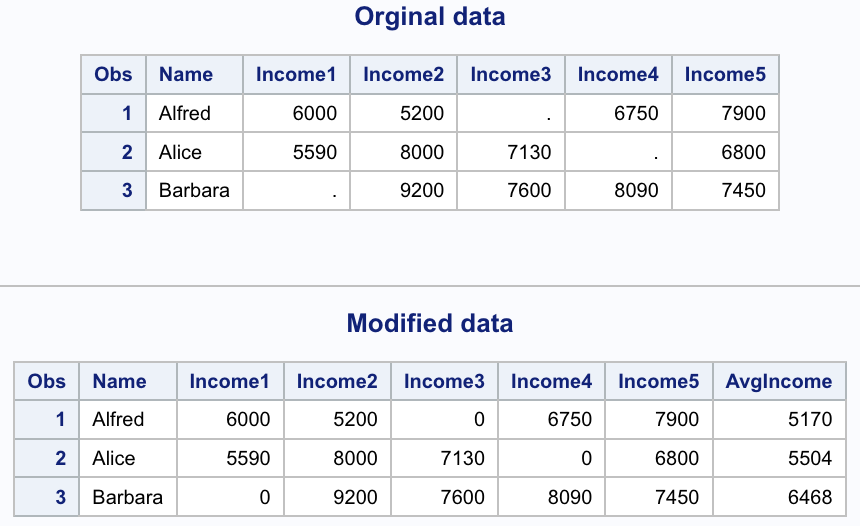
\includegraphics[scale=0.6]{DataStep-Arrays.png}
\end{figure}
	
\section{Combining data}

\subsection{Concatenating}
\begin{itemize}
\item Uses a SET statement to concatenate datasets one after the other.
\item If datasets have different variables, SAS will create missing values in the uncommon columns for all of the rows.
\end{itemize}
\lstinputlisting{Combining-Concatenating.txt}

\subsection{Interleaving}
\begin{itemize}
\item Arranges rows by the values of the BY variable, by the order of the datasets in which they occur.
\item Uses a SET statement with a BY statement.
\item Datasets must be sorted by the BY variable.
\end{itemize}
\lstinputlisting{Combining-Interleaving.txt}

\subsection{Combining rows (one-to-one)}
\begin{itemize}
\item Combines the first observation from all the datasets into the first observation of the new dataset, the second row in all datasets into the second row in the new dataset, and so on.
\item Uses several SET statements.
\item If datasets have the same variables, the values that are read in from the last dataset will replace the values that are read in from earlier datasets.
\end{itemize}
\lstinputlisting{Combining-Combining1to1.txt}

\subsection{Match merging}

Overall -> All three types of match merging:
\begin{itemize}
\item Combine datasets based on a common variable (could be multiple).
\item Use a MERGE statement.
\item Two or more datasets must be listed in the MERGE statement.
\item Variables in the BY statement must be common to all datasets.
\item Datasets must be sorted by the variables listed in the BY statement.
\item The order of datasets in the MERGE statement doesn't impact results, just the order of the variables in the new dataset will differ.
\end{itemize}

One-to-one:
\begin{itemize}
\item Use when a single observation in one dataset is related to exactly one observation in another dataset based on the BY values (i.e. BY values have only one match in the other datasets).
\end{itemize}

One-to-many:
\begin{itemize}
\item Use when a single observation in one dataset is related to more than one observation in another dataset based on the BY values (i.e. BY values have multiple matches in the other datasets).
\end{itemize}

\lstinputlisting{Combining-MatchMerging.txt}

Non-matches:
\begin{itemize}
\item Use when at least one observation in one dataset is unrelated to any observation in another dataset based on the BY values (i.e. BY values do not have to have a match in the other datasets).
\item The in= dataset option creates a temporary numeric variable that indicates whether
that dataset contributed to building the current observation of the new dataset.
	\begin{itemize}
	\item \textit{invar}=0 if that dataset did not contribute and 1 if it did.
	\item Helpful when you want to perform some action based on which dataset an observation came from (e.g. subsetting new dataset to only observations from certain datasets; or keeping only records with a match).
	\item \textit{invar} is only available during the DATA step in which it occurs -> So if it is needed for later DATA steps, it needs to be assigned to another variable.
	\end{itemize}
\end{itemize}
	
\lstinputlisting{Combining-MatchMerging-Non.txt}
	
\section{Export and write}

\subsection{Datasets}

\lstinputlisting{ExWrite-Datasets-ProcExport.txt}
\lstinputlisting{ExWrite-Datasets-Ods.txt}

\subsection{Output}

\lstinputlisting{ExWrite-Output.txt}

\subsection{Reports with put statement}

\begin{itemize}
\item \_NULL\_ dataset allows for a DATA step without storing the dataset.
\item PUT statement writes to the SAS log.
\item If FILE statement is specified, then PUT writes to the specified location.
\item MOD option in the FILE statement appends text to the end of the file.
\item Do not need to put \$ to indicate character variables and can also specify formats after variables.
\item Can use column pointer controls to organize report.
\item Can use multiple put statements (e.g. if want to add a line of string constants).
\item To make an overall header for the report, you can use two DATA steps:
	\begin{itemize}
	\item The first only has the FILE statement and the PUT statements that write the header.
	\item Then the second on actually has the dataset and the FILE statement with the MOD option so that you can append the actual report.
	\end{itemize}
\item If want to organize report by a BY variable:
	\begin{itemize}
	\item Need to sort the data by the BY variable and add a BY statement to the DATA step.
	\item Then can use if first.\textit{byvar} and add a header for the BY group and if last.\textit{byvar} to separate groups.
	\end{itemize}
\end{itemize}
\lstinputlisting{ExWrite-ReportsWithPut-General.txt}
\lstinputlisting{ExWrite-ReportsWithPut-Example.txt}
\begin{figure}[H]
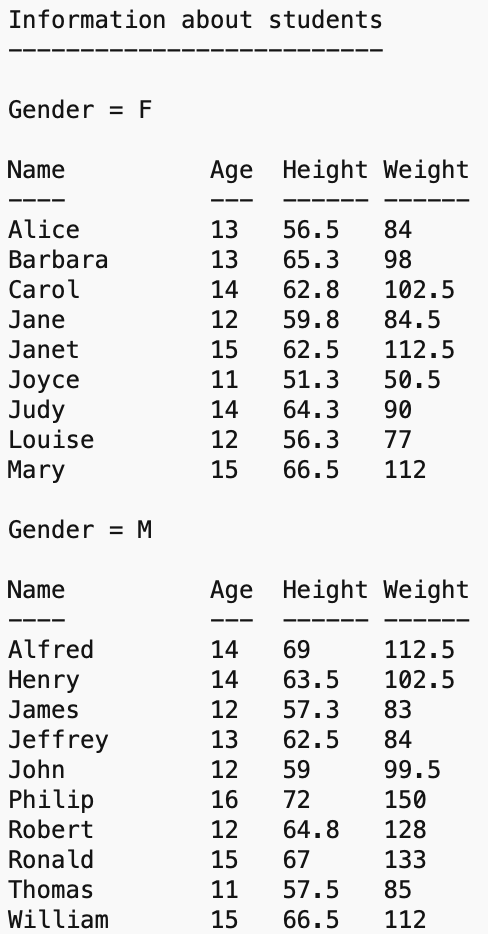
\includegraphics[scale=0.6]{ExWrite-ReportsWithPut.png}
\end{figure}

\section{Proc procedures}

Here are notes about some PROC procedures...

\subsection{Proc sql}

SQL (Structure Query Language):
\begin{itemize}
\item Can sort, summarize, subset, join (merge), concatenate datasets, create new variables, print results or create a new table all in a single step.
\item Terminology (SAS <--> SQL equivalent):
	\begin{itemize}
	\item Dataset <--> Table.
	\item Observation <--> Row.
	\item Variable <--> Column.
	\end{itemize}
\item Can add multiple CREATE TABLE, SELECT, etc. statements within a single PROC SQL step.
\item The SQL procedure is finished after the QUIT statement.
\end{itemize}

\lstinputlisting{Proc-Sql.txt}

\subsection{Proc report}	

Options:
\begin{itemize}
\item HEADLINE adds a line after the column headings.
\item HEADSKIP option adds a blank line under the column heading (or line from above option).
\end{itemize}
TITLE statement:
\begin{itemize}
\item Used to specify the title at the top of each page.
\end{itemize}

COLUMN statement:
\begin{itemize}
\item Used to list each report column.
\item By default, column headings are their respective labels, not the variable names. 
\end{itemize}

DEFINE statement:
\begin{itemize}
\item Each column then has a DEFINE statement that describes how that column is created and formatted (via slash / options).
\item Define types:
	\begin{itemize}
	\item The word directly after the slash specifies the define type for that column.
	\item DISPLAY:
		\begin{itemize}
		\item Simply displays the column.
		\end{itemize}
	\item ORDER:
		\begin{itemize}
		\item Specifies the column used to sort the report. 
		\end{itemize} 
	\item GROUP:
		\begin{itemize}
		\item Aggregates all the observations with the same unique combination of grouped variables.
		\item Not very useful unless it is used with the ANALYSIS define type.
		\item You can specify the order of the rows within the group by using the ORDER= option of the DEFINE statement.
		\end{itemize}
	\item ANALYSIS:
		\begin{itemize}
		\item Lets you specify for that column any of the statistics used in PROC MEANS, SUMMARY and UNIVARIATE.
		\item The statistics are calculated for the group you defined.
		\item If you want to calculate more than one statistic on the same column, you create an alias in the COLUMN statement (\textit{column=columnalias}). 
		\end{itemize}
	\item ACROSS:
		\begin{itemize}
		\item Use when you want a report where all the unique values of a variable have their own column.
		\item This is the easiest way to create cross-tab.
		\item Can specify a variable to be nested under the across variable by separating the across variable and the nested variable with a comma in the COLUMN statement.
		\item If you use dashes (or some other character) as the first and last characters in the ACROSS column header, they span all the columns.
		\end{itemize}
	\item COMPUTED:
		\begin{itemize}
		\item Used to compute your own values from the other data in your report.
		\item Besides the DEFINE statement for each computed column, you need to write a COMPUTE block which starts with a COMPUTE statement and ends with ENDCOMPUTE.
		\item A COMPUTE block can contain, more or less, everything allowed in a DATA step including macro variables and \%INCLUDE (can also reference any report item from within the block). 
		\item Can use the automatically defined \_C\#\_ variables to make it easier (e.g. sum(\_C2\_, \_C3\_, \_C5\_) is the sum of the second, third and fifth columns). 
		\item If don't know how many columns ACROSS define type will create, just use a really big \_C\#\_ (extra variables won't hurt).
		\end{itemize}
	\end{itemize}
\item Formatting options:
	\begin{itemize}
	\item FORMAT= applies the standard SAS formats to the column.
	\item WIDTH= sets the width of the column. 
	\item FLOW wraps the text within the width you specified.
	\item NOPRINT suppresses printing that column.
	\item You can replace the label as the column heading by specifying the new heading in quotes (use a / to insert a line break).
	\end{itemize}
\end{itemize}

BREAK and REBREAK statements:
\begin{itemize}
\item BREAK adds summaries (subtotals in this case) every time the group column(s) change.
\item REBREAK gives you grand totals.
\item You can specify whether the break occurs before or after the group.
\item There are many options for these:
	\begin{itemize}
	\item OL -> Overline.
	\item DOL -> Double overline.
	\item UL -> Underline.
	\item DUL -> Double underline.
	\item SUMMARIZE -> Summarize each group.
	\item SKIP -> Skip a line after the break.
	\item SUPPRESS -> Don?t repeat the break variable on the summary line.
	\end{itemize} 
\end{itemize}

\lstinputlisting{Proc-Report.txt}

\subsection{Proc format}

\begin{itemize}
\item Used to create custom formats and informats.
\item Use an INVALUE statement for informats and a VALUE statement for formats.
\item If the original value is a character, then you need to specify the \$.
\item Setting ranges:
	\begin{itemize}
	\item a - b: a <= var <= b.
	\item a <- b: a < var <= b.
	\item a -< b: a <= var < b
	\item a <-< b: a < var < b.
	\item Can also use low and high.
	\item Can also specify missing values (.=) and other values (other=).
	\end{itemize}
\end{itemize}
\lstinputlisting{Proc-Format.txt}
\begin{figure}[H]
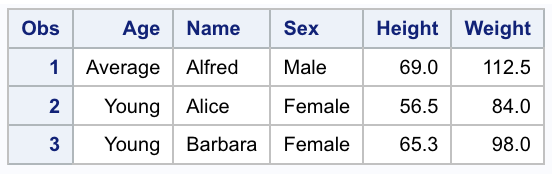
\includegraphics[scale=0.6]{Proc-Format.png}
\end{figure}

\subsection{Proc iml}

IML (Interactive Matrix Language):
\begin{itemize}
\item The IML procedure is finished after the QUIT statement.
\end{itemize}

Syntax:
\begin{itemize}
\item Initialize vector -> \textit{vector}=\{\textit{values}\}.
\item Print vector -> print \textit{vector}.
\end{itemize}

Operators:
\begin{itemize}
\item To perform calculations:
	\begin{itemize}
	\item Addition +.
	\item Subtraction -.
	\item Multiplication *.
	\item Division /.
	\item Switch sign -.
	\item Power **.
	\item Multiplication (elementwise) \#.
	\item Power (elementwise) \#\#.
	\end{itemize}
\item To modify:
	\begin{itemize}
	\item Subscripts [].
	\item Horizontal concatenation ||.
	\item Vertical concatenation //.
	\item Transpose <accent mark (the one on the tilde key)>.
	\end{itemize}
\end{itemize}

Functions:
\begin{itemize}
\item J(\textit{nrow(, ncol, value)}):
	\begin{itemize}
	\item Creates a matrix that has \textit{nrow} rows, \textit{ncol} columns, and all elements equal to \textit{value}.
	\item \textit{ncol} and \textit{value} arguments are optional;
	\end{itemize}
\item I(\textit{dimension}):
	\begin{itemize}
	\item Creates an identity matrix of a given size.
	\end{itemize}
\item REPEAT(\textit{matrix, nrow, ncol}):
	\begin{itemize}
	\item Creates a new matrix by repeating elements of \textit{matrix}.
	\end{itemize}
\item SHAPE(\textit{matrix, nrow(, ncol, padvalue})):
	\begin{itemize}
	\item Creates a new matrix by reshaping \textit{matrix}.
	\item Cycles back and repeats values to fill in the matrix when no pad value is given.
	\item Cycles through \textit{matrix} elements in row-major order and fills in the new matrix with \textit{padvalue} after the first cycle through \textit{matrix}.
	\end{itemize}
\end{itemize}

Random number generation (example):
\begin{enumerate}
\item Allocate a vector with \textit{vector}=j(\textit{nrow(, ncol, initial value)}).
\item Fill vector with call randgen(\textit{vector}, \textit{distribution, parameter1, ...}): 
\end{enumerate}

\section{Macro language}

\subsection{Macro definition and calling}

\begin{itemize}
\item Define a macro with \%MACRO and \%MEND.
\item Call a macro with \%\textit{macroname} (using a semicolon following a macro call is not recommended and can cause problems).
\end{itemize}
\lstinputlisting{MacLang-DefCall.txt}

\subsection{Macro variables}

\begin{itemize}
\item Help to make macros more dynamic and flexible.
\item Refer to a macro variable with \&\textit{macrovar}.
\item Global macro variables:
	\begin{itemize}
	\item Defined outside of a macro with a \%LET statement.
	\item Exist for the remainder of the current SAS session.
	\end{itemize}
\item Local macro variables:
	\begin{itemize}
	\item Defined within a macro and are not specifically defined as global.
	\item Exist only during execution of the macro in which they are defined.
	\end{itemize}
\end{itemize}

\subsection{Macro parameters}

Parameter lists are a list of macro variables referenced within the macro. There are two types: positional and keyword (can also use both at once for a mixed parameter list, but kind of confusing).

Positional parameters:
\begin{itemize}
\item Define macro parameters in a particular order.
\item Parameter names are supplied when the macro is defined.
\item Parameter values are supplied when the macro is called (and they must appear in the same order as their corresponding parameter names).
\end{itemize}

Keyword parameters:
\begin{itemize}
\item Assigned a default value after an equal sign.
\item Can appear in any order and can be omitted from the call without placeholders.
	\begin{itemize}
	\item If omitted from the call, a keyword parameter receives its default value.
	\end{itemize}
\end{itemize}
\lstinputlisting{MacLang-Parameters.txt}

Parameter validation (two methods):
\begin{enumerate}
\item Use the IN operator (the MINOPERATOR option is required).
\item Use data-driven parameter validation.
	\begin{itemize}
	\item Useful when the list of valid parameters is extremely long or changes frequently.
	\item Uses PROC SQL to create macro variables that contain values from a query result.
	\end{itemize}
\end{enumerate}
\lstinputlisting{MacLang-Parameters-Valid.txt}

\subsection{Conditional processing and iterative statements}

Conditionally process portions of a macro:
\begin{itemize}
\item Uses \%IF, \%THEN, and \%ELSE statements.
\item The macro language does not contain a subsetting \%IF statement, so you cannot use \%IF without \%THEN.
\item Difference between  \%IF-\%THEN/\%ELSE and IF-THEN/ELSE:
	\begin{itemize}
	\item The macro ones conditionally generate text, while the other conditionally executes SAS statements during DATA step execution.
	\end{itemize}
\end{itemize}

Iterative statement:
\begin{itemize}
\item Executes a section of a macro repetitively based on the value of an index variable. 
\item Uses \%DO loops (so can use \%TO, \%UNTIL or \%WHILE loops).
\end{itemize}

\lstinputlisting{MacLang-ConditionalIterative.txt}

\subsection{Macro functions}

Here are some functions related to macro variables (they can be used outside of a DATA / PROC step)...

\%EVAL(\textit{expression}):
\begin{itemize}
\item Evaluates integer arithmetic or logical expressions (will return a 0 for false and a 1 for true).
\item Discards the fractional part when it performs division on integers that would result in a fraction.
\item Expression can only contain integers.
\end{itemize}

\%INCLUDE:
\begin{itemize}
\item Brings a SAS programming statement, data lines, or both, into a current SAS program.
\item Allows you to run another SAS program (in an external file) without having to have it all typed out in the current session (i.e. saves typing and helps organization).
\end{itemize}

\%PUT:
\begin{itemize}
\item Writes macro variable values as text in the SAS log.
\item Can include regular text as well (do not need quotes surrounding text).
\item If you place an equal sign between the ampersand and the macro variable name of a direct macro variable reference, the macro variable's name is displayed in the log along with its value (e.g. \%PUT \&=x writes X=\textit{value} to the log).
\end{itemize}

\%SCAN(\textit{var,k}):
\begin{itemize}
\item Returns the $k$th word from var (if k<0, counts from right to left).
\end{itemize}

\%SUBSTR(\textit{var,start,length}):
\begin{itemize}
\item Returns the parsed string of \textit{var} (starting from \textit{start} and \textit{length} characters long).
\end{itemize}

\%SYMGET(\textit{macrovar}):
\begin{itemize}
\item Returns the value of a macro variable to the DATA step during DATA step execution.
\item There are variations of SYMPUT for different types of \textit{value}.
\end{itemize}

\%CALL SYMPUT(\textit{macrovar,value}):
\begin{itemize}
\item Assigns a value produced in a DATA step to a macro variable. 
\item \textit{macrovar}:
	\begin{itemize}
	\item Most useful when \textit{macrovar} is a variable name (or an expression containing a variable name) because a unique macro variable can be created and assigned a value from each observation.
	\item If \textit{macrovar} is a character string, SYMPUT creates only one macro variable, and its value changes in each iteration of the program. Only the value assigned in the last iteration remains after program execution is finished.
	\end{itemize}
\item || (concatenation operator):
	\begin{itemize}
	\item Concatenates character values.
	\item Useful when making macro variable names.
	\end{itemize}
\item There are variations of SYMPUT for different types of \textit{value}.
\end{itemize}

\%SYSEVALF(\textit{expression, conversion type}):
\begin{itemize}
\item Same thing as \%EVAL, except it can have decimals in the expression and keeps the decimals in the result.
\item Conversion type can be: BOOLEAN, CEIL, FLOOR or INTEGER.
\end{itemize}

\%UPCASE:
\begin{itemize}
\item Returns a string in all caps.
\end{itemize}
	
\subsection{Resolving macro variables}

Rules for processing consecutive ampersands:
\begin{enumerate}
\item Two ampersands always resolve (simplify) to one ampersand.
\item The macro processor continues to read left to right until the end of the reference is reached.
	\begin{itemize}
	\item i.e. The single ampersand that results from two from Rule 1 is left alone as the macro processor reads left to right, and will not be processed until a subsequent read.
	\item So with $n$ ampersands, ampersands one and two resolve to one, then three and four resolve to one, and so on.
	\item The macro processor will then go back and re-process those results only after the entire reference has been processed initially;
	\end{itemize}
\item When a reference contains consecutive ampersands, after resolution, at least one more read will follow (this is the only way to force more reads by the macro processor).
\end{enumerate}

Notation and example:
\begin{itemize}
\item If \&a resolves to b, then it can be written as \&a => b.
\item ($n$)a denotes that the macro variable a is preceded by $n$ ampersands ($n$ is referred to as the coefficient of the macro variable).
\item For illustration purposes, assume:
	\begin{itemize}
	\item \&a => b.
	\item \&b => c.
	\item \&c => d.
	\item \&d => e.
	\item etc.
	\end{itemize}
\end{itemize}
	
Macro variable references of the form ($n$)a:
\begin{itemize}
\item With $n=2$, \&\&a => \&a => b.
	\begin{itemize}
	\item This is because of Rule 1.
	\item The only difference between  \&\&a and \&a is one more read, but the end 	result is the same.
	\item So in this case, the extra ampersand adds no value (i.e. $n=2$ is not a useful coefficient of a).
	\end{itemize}
\item With $n=3$, \&\&\&a => \&b => c.
	\begin{itemize}
	\item Rule 1 says that the first two resolve to a single ampersand, and Rule 2 says that the third is used to resolve a.
	\item i.e. After the first read you are left with the single ampersand that came from the first two of the original reference, plus the resolution of a (which is b). A second read would then resolve b.
	\end{itemize}
\item So, when the possible values of a macro variable are also macro variables, repeated ampersands creates a chain effect of macro variable resolution.
	\begin{itemize}
	\item However only some numbers of $n$ are useful.
	\end{itemize}
\end{itemize}

Patterns when the initial reference (prior to any read) shows only one ampersand:
\begin{itemize}
\item When $n$ is even, the macro variable does not get resolved on that read (i.e. not useful).
\item So useful coefficients are odd numbers of $n$ that resolve to something unique.
	\begin{itemize}
	\item (1)a => b.
	\item (3)a => (1)b => c.
	\item (7)a => (3)b => (1)c => d.
	\item And so on...
	\end{itemize}
\end{itemize}

Macro variable references of other forms:
\begin{itemize}
\item ($n$)a\&b, where $n$ is even and a is not a macro variable.
	\begin{itemize}
	\item The effect of the even coefficient is a delayed resolution.
	\item On the first read, the macro processor resolves the $n$ ampersands to $n/2$ ampersands (because of Rule 1) and also resolves \&b.
	\item Thus, you are left with $(n/2)$ ampersands and the name of a new macro variable, the concatenation of a and simplified \&b.
	\item So, useful coefficients of the form ($n$)a\&b are equivalent to twice the useful coefficients of the form ($n$)a.
	\end{itemize}
\item There are many other helpful forms...
\end{itemize}

Another special character:
\begin{itemize}
\item Wherever an ampersand shows up, the macro processor will try to resolve anything that follows, including within a string of text not meant to be resolved. 
\item So if a macro variable reference is at the beginning of a text string...
	\begin{itemize}
	\item Use a period as a delimiter to signify the end of a macro variable reference.
	\item If multiple reads are necessary for resolving the macro variable immediately before the text string, then you need that many periods.
	\item If want a period in the end result (such as a filename), then just use an extra one. 
	\end{itemize}
\end{itemize}

\subsection{Options}

Use these in OPTIONS statement to help debug macros.
\begin{itemize}
\item Specified options remain in effect for the rest of the SAS session or until you issue another OPTIONS statement to change the options again.
\end{itemize}

MCOMPILENOTE=ALL:
\begin{itemize}
\item Used to verify macro compilation.
\end{itemize}

MPRINT:
\begin{itemize}
\item Used to view the text generated by macro execution (gets output to SAS log).
\item i.e. Translates process from a macro program to regular SAS statements.
\end{itemize}

MLOGIC:
\begin{itemize}
\item If a macro is invoked, this option displays messages that identify the following:
	\begin{itemize}
	\item The beginning of macro execution.
	\item Values of macro parameters at invocation.
	\item Execution of each macro program statement.
	\item Whether each \%IF condition is true or false.
	\item The ending of macro execution.
	\end{itemize}
\item Note -> This produces a lot of output, so only try it on test runs.
\end{itemize}

SYMBOLGEN:
\begin{itemize}
\item Displays the results of resolving macro variable references.
\item Useful for debugging.
\end{itemize}

\subsection{Macro storage}

Submitting a macro definition causes the following actions:
\begin{enumerate}
\item The macro is compiled.
	\begin{itemize}
	\item Macro language statements or expressions are checked for syntax errors and then compiled.
	\item SAS statements and other text are not checked for syntax errors and are not compiled.
	\end{itemize}
\item The macro is stored.
	\begin{itemize}
	\item By default, the compiled macro is stored in the temporary catalog work.sasmacr, with an entry type of MACRO.
	\end{itemize}
\end{enumerate}

Saving macros using the stored compiled macro facility:
\begin{itemize}
\item Contains permanently compiled macros (and may or may not have source code stored in the same directory).
\item The compiled macros can be seen in the SAS macro catalog SASMACR.
\item Advantages of storing already compiled macros:
	\begin{itemize}
	\item Decreased processing time, the macro will be the same every time it is run, and users are not able to modify the macro.
	\item i.e. Reports and analysis produced with these macros will be consistent.
	\end{itemize}
\item Strategy for saving macro:
	\begin{itemize}
	\item Create a folder where SAS will store the catalog SASMACR.
	\item Assign a library to that folder with a LIBNAME statement.
	\item Then submit the macro definitions that you want to go in there by adding the STORE option to the macros.
	\item Can make the source code of the macro available by adding the SOURCE option.
	\item Can also add descriptions to the macros with the DES= option.
	\end{itemize}
\item Strategy for using stored macros:
	\begin{itemize}
	\item Just have to run the OPTIONS and LIBNAME statement used to save the macro.
	\item Then you are able to use those macros as if they were submitted in the current session.
	\item Can view all stored macros with PROC CATALOG and CONTENTS statement.
	\item Can delete a macro from the catalog by using a DELETE statement. 
	\end{itemize}
\end{itemize}

\lstinputlisting{MacLang-Storing.txt}

\section{Reusable macros}

The code below shows where these macros are stored in addition to more related code:
\lstinputlisting{ReuseMac-Store.txt}

\subsection{Reshape dataset from wide to long}

\%wideToLong:
\begin{itemize}
\item Purpose:
	\begin{itemize}
	\item Reshape dataset from wide to long.
	\end{itemize}
\item Arguments:
	\begin{itemize}
	\item wideData -> Input dataset (wide).
	\item longData -> Output dataset (long).
	\item stackVars -> List of variables to be stacked.
	\item keepRow:
		\begin{itemize}
		\item 0 (no) or 1 (yes, default).
		\item Specifies whether or the row index should be kept in the output dataset.
		\item Tip -> Set to 0 if transposing a row vector.
		\end{itemize}
	\item keepVars:
		\begin{itemize}
		\item List of additional variables to keep in output dataset.
		\item Tip -> Do not need to supply an argument if only the stacked variables are wanted.
		\end{itemize}
	\end{itemize}
\item Call:
	\begin{itemize}
	\item Can rename the row index, column index and newly created variable with a RENAME= option for the output dataset.
		\begin{itemize}
		\item rowIndex -> Identifier for which observation is being read from the input dataset.
		\item colIndex -> Identifier for which column (of the stacked vars) is being read from the input dataset.
		\item newVar -> Newly created column of the values of the stacked vars.
		\item Tip -> If keepRow=0 then do not need to RENAME= option for rowIndex.
		\end{itemize}
	\end{itemize}
\end{itemize}

\lstinputlisting{ReuseMac-wideToLong.txt}

\subsection{Get info about dataset}
\begin{itemize}
\item Purpose:
	\begin{itemize}
	\item Get info about dataset.
	\end{itemize}
\item Arguments:
	\begin{itemize}
	\item what:
		\begin{itemize}
		\item nobs or vars.
		\item Specifies whether to perform process to view number of observations (nobs) or variables (vars).
		\end{itemize}
	\item inData -> Input dataset.
	\end{itemize}
\end{itemize}

\lstinputlisting{ReuseMac-info.txt}

\section{Simulation}

\subsection{Inner workings and implicit / explicit output statements}

Inner workings of SAS:
\begin{itemize}
\item There is an implicit looping mechanism in SAS, so when no input dataset is specified, the DATA step only executes once. But when there is an input dataset with $n$ observations, the DATA step executes $n$ times (once through for each observation).
\end{itemize}

Implicit / explicit output statements:
\begin{itemize}
\item If there is no OUTPUT statement, SAS does an implicit OUTPUT statement at the end of a DATA step.
	\begin{itemize}
	\item So if use DO loop to generate random numbers and do not have an OUTPUT statement, there will only be one observation because the DATA step is only executed once.
	\end{itemize}
\item So, with a DO loop you have to use an explicit OUTPUT statement, which causes SAS to write the current observation.
	\begin{itemize}
	\item When there is an explicit OUTPUT statement, SAS no longer executes the implicit one.
	\end{itemize}
\end{itemize}

\subsection{Random number generation}

CALL STREAMINIT(\textit{seed}):
\begin{itemize}
\item Sets random seed.
\end{itemize}

RAND(\textit{distribution, parameter1, ...}):
\begin{itemize}
\item Use this function to generate random numbers from a known distribution.
\item May need to perform additional operations to add a location or rate/scale parameter.
	\begin{itemize}
	\item Location -> RAND(<...>) + \textit{location param}.
	\item Rate -> RAND(<...>) / \textit{rate param}.
	\item Scale -> RAND(<...>) * \textit{scale param}.
	\item Note -> Scale = 1/Rate.
	\end{itemize}
\end{itemize}

\lstinputlisting{Sim-RandomNum.txt}
\begin{figure}[H]
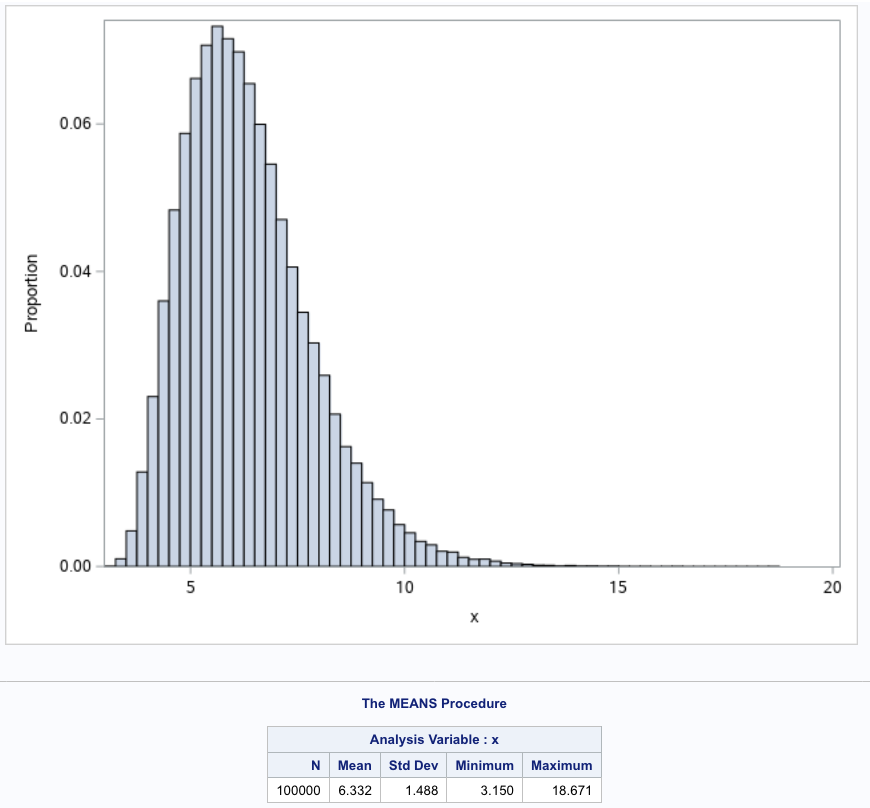
\includegraphics[scale=0.6]{Sim-RandomNum.png}
\end{figure}

\subsection{Simulating methods}

General logic:
\begin{enumerate}
\item Figure out the model and generate many samples.
	\begin{itemize}
	\item Model depends on the experiment you are simulating (e.g. could be a binomial experiment or values assumed to come from exponential distribution, or etc.).
	\item Output after each simulation (i.e. after each sample is generated).
	\end{itemize}
\item Calculate statistics for each sample.
	\begin{itemize}
	\item Use arrays and of to perform calculations over the entire row.
	\end{itemize}
\item Accumulate results over all the simulated datasets.
	\begin{itemize}
	\item Can use PROC MEANS or PROC UNIVARIATE to summarize results. Can also plot results with PROC SGPLOT.
	\end{itemize}
\end{enumerate}

Data structure:
\begin{itemize}
\item Rows:
	\begin{itemize}
	\item Represent the different simulations (i.e. the first row is the first sample, the second row is the second sample, ...).
	\item Number of rows is equal to the number of simulations or samples.
	\end{itemize}
\item Columns:
	\begin{itemize}
	\item Represent individual observations (i.e the fifth column of the third row is the fifth observation of the third sample).
	\item Number of columns is equal to the sample size.
	\end{itemize}
\end{itemize}

Example -> Simulation study of one-proportion z-test:
\begin{itemize}
\item Test whether a proportion is equal to a hypothesized proportion.
\item Hypotheses -> $H_0\rightarrow p=0.8\quad\&\quad H_A\rightarrow p\ne0.8$.
\item This example calculates the power of the test if the true proportion is 0.1 less than the hypothesized proportion.
\item < test statistic distribution, p-value calculation formula and decision rule >.
\end{itemize}
\lstinputlisting{Sim-Methods.txt}
\begin{figure}[H]
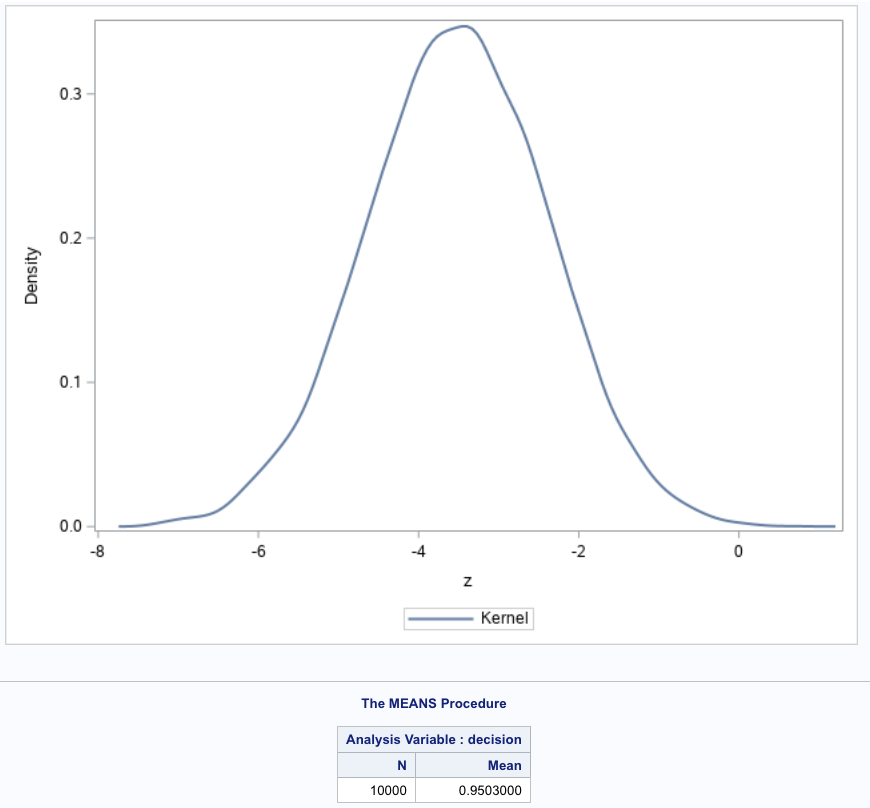
\includegraphics[scale=0.6]{Sim-Methods.png}
\end{figure}

\subsection{Bootstrapping}

General logic:
\begin{enumerate}
\item Create dataset of original sample.
	\begin{itemize}
	\item Assign number of observations to a macro variable with SYMPUTX (use variation to remove extra blanks).
	\item Transpose sample into a row vector (PREFIX option specifies prefix for created variables and VAR statement specifies the column to transpose). 
	\end{itemize}
\item Create bootstrap samples by sampling with replacement from the original sample (also calculate desired statistic for each sample).
\item Create confidence intervals.
	\begin{itemize}
	\item PCTLPTS option specifies additional percentiles that aren't automatically computed by PROC UNIVARIATE.
	\item PCTLPRE option specifies prefixes of variables in the output dataset.
	\item Note -> These options must be used together.
	\end{itemize}
\end{enumerate}

\lstinputlisting{Sim-Boot.txt}
\begin{figure}[H]
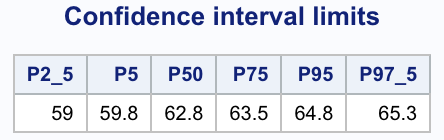
\includegraphics[scale=0.6]{Sim-Boot.png}
\end{figure}

\section{Miscellaneous}

\subsection{Libraries}

\lstinputlisting{Misc-Libraries.txt}

\subsection{Converting data types}

To convert character values to numeric values, use the INPUT function.
\begin{itemize}
\item Syntax -> \textit{newvar} = input(\textit{original variable, informat.});
\end{itemize}

To convert numeric values to character, use the PUT function:
\begin{itemize}
\item \textit{newvar} = put(\textit{original variable, format.});
\end{itemize}

\subsection{Dates}

\begin{itemize}
\item SAS stores dates as the number of days from January 1, 1960.
\item In order to tell SAS about a specific date, you need to use literals.
	\begin{itemize}
	\item Date literals have the form 'ddmmmyyyy'd.
	\item Time literals have the form 'hh:mm:ss't (based on 24 hour clock).
	\item Datetime literals have the form 'ddmmmyyyy:hh:mm:ss'dt (based on 24 hour clock).
	\end{itemize}
\end{itemize}

\subsection{Special characters in plot titles / axis labels}

\begin{itemize}
\item Use ODS ESCAPECHAR='\textasciitilde' statement.
\item Then for desired string, use "\textasciitilde\{unicode '03BB'x\}" (03BB is for $ \lambda$, so that will change).
\end{itemize}

\subsection{Sources and resources}

% replace ~ with \%7e and a space with \%20
\begin{itemize}
\item \href{https://documentation.sas.com/?cdcId=pgmsascdc\&cdcVersion=9.4\_3.4\&docsetId=pgmsashome\&docsetTarget=home.htm\&locale=en}{\color{blue}New SAS documentation (Has good stuff for PROC procedures).}
\item \href{https://documentation.sas.com/?cdcId=pgmsascdc\&cdcVersion=9.4\_3.4\&docsetId=odsproc\&docsetTarget=p037wkiv6e4hqln1snmfk9b7c9it.htm\&locale=en}{\color{blue}ODS table names.}
\item \href{https://support.sas.com/resources/papers/proceedings09/060-2009.pdf}{\color{blue}Proc transpose.}
\item \href{http://www2.sas.com/proceedings/forum2008/079-2008.pdf}{\color{blue}Proc report.}
\item \href{http://www2.sas.com/proceedings/sugi29/063-29.pdf}{\color{blue}Resolving macro variables.}
\end{itemize}

\section{Application}

\subsection{Example 1}

\lstinputlisting{Example-1.txt}

\subsection{Example 2}

\lstinputlisting{Example-1.txt}

\subsection{Final report}

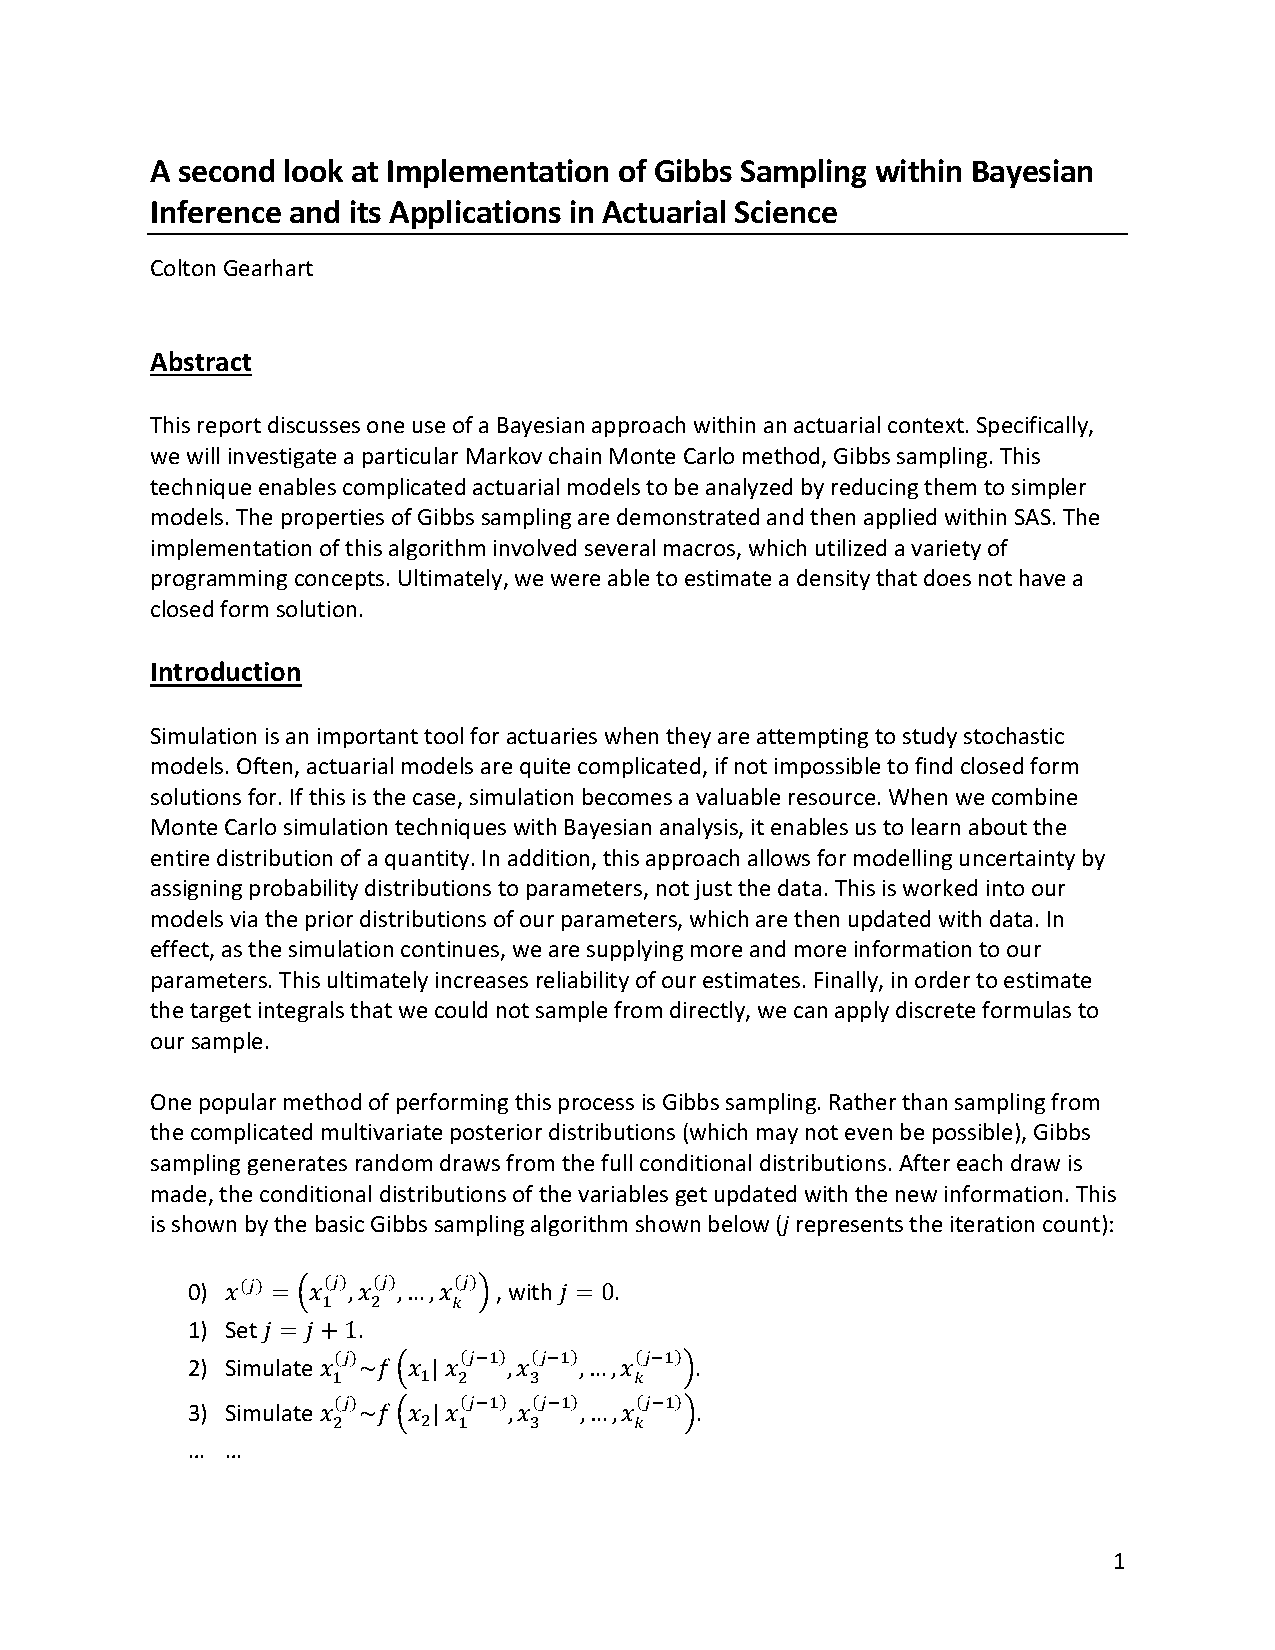
\includepdf[pages=-]{Files/Final-report.pdf}

\end{document}